% myelin water fraction estimation from steady state sequences

%%%%%%%%%%%%%%%%%%%%%%%%%%%%%%%%%%%%%%%%%%%%%%%%%%%
\section{Introduction}
\label{s,mwf,intro}
%%%%%%%%%%%%%%%%%%%%%%%%%%%%%%%%%%%%%%%%%%%%%%%%%%%

This chapter applies techniques
(developed in earlier chapters)
for QMRI acquisition design
and parameter estimation
to design new methods 
for imaging a specific MR biomarker
of clinical interest.
In particular,
we study a biomarker 
for \emph{myelin content} 
in the human brain.

Myelin is a lipid-rich material
that forms an insulating sheath
encasing neuronal axons 
predominantly in white matter (WM) regions
of the human brain
\cite{morell:84}.
Demyelination (\ie, myelin loss) is central
to the development 
of several neurodegenerative disorders
such as multiple sclerosis (MS)
\cite{goldenberg:12:msr}. 
Non-invasive myelin quantification in WM
is thus desirable 
for monitoring the onset and progression
of neurodegenerative disease.

% MR relaxation rates (esp t2) depend on water environment
% local water environment changes on sub-millimeter scale
% MR sensitive only on millimeter scale
% need to assign a macroscopic t2 to each pool or compartment
% thus multiple water compartments contribute to each voxel at typical resolutions
MR relaxation time constants
(especially spin-spin time constant $\Tt$)
depend on the macromolecular environment
surrounding excited water molecules.
In nervous tissue,
these environments vary spatially
on scales much smaller 
than the millimeter-scale resolutions
used in typical MR imaging experiments.
Thus, 
there is significant variation
of relaxation times 
within a typical imaging voxel 
containing nervous tissue.

% natural to try to separate t2 components in mri
% several groups measured first in vitro short t2 pool in white matter
% assigned to water in myelin (trapped in bilayers?)
% later measured in vivo, who termed mwf (mackay)
% mwf found to correlate well in vivo with histology (laule)
% mwf thus noninvasive MR-based biomarker for myelin content
Many researchers have attempted 
to characterize tissue microstructure
by estimating the distribution
of MR relaxation time constants
and associating certain ranges of time constants
with particular ``compartments'' or ``pools'' of water molecules
that exist in similar macromolecular environments.
\emph{In vitro} NMR studies
of nervous animal tissue
ascribed a fast-relaxing
\footnote{The fast-relaxing compartment bears its name 
	with reference to the portion 
	of the $\Tt$ distribution in water
	(from about $10$ms to at least $1000$ms)
	that is typically observable in MRI.
}
water compartment
with $\Tt\sim$10-40ms 
initially to general protein 
and phospholipid structures \cite{vasilescu:78:wci}
and later more specifically
to water trapped between
the phospholipid bilayers 
of myelin
\cite{menon:91:aoc, stewart:93:ssr}.
Shortly thereafter,
the first MR images 
of so-called \emph{myelin water fraction} (MWF),
defined as the proportion of MR signal 
arising from the fast-relaxing water compartment
relative to total MR signal,
were demonstrated \emph{in vivo}
in the human brain \cite{mackay:94:ivv}.
More recently,
MWF has been shown 
to correlate well 
with histological measurements
of myelin content 
in animal models
of nerve injury \cite{gareau:00:mta}
and demyelination \cite{webb:03:imt}.
In humans, 
MWF has also been measured 
to be markedly lower
in ``normally appearing'' WM 
of MS patients versus controls \cite{laule:04:wca},
and to correlate strongly 
with post-mortem histological measurements
of myelin content
in MS patients \cite{laule:06:mwi}.
Thus,
there is reasonably strong evidence
that MWF
(as defined in \cite{mackay:94:ivv})
is a specific and non-invasive biomarker
for myelin content in WM.

% all aforementioned studies used MESE 
% MESE typically uses long tr to ensure full recovery between excitations
% thus MESE acquisitions take long time
% mcdespot based on ss techniques (specifically spgr and bssfp) 
% shown to disagree significantly with ss 
% maybe due to insufficient precision
All of the aforementioned studies
estimate MWF images
from a multi-echo spin echo (MESE) MRI pulse sequence
\cite{carr:54:eod}
with long repetition time $\TR\geq2$s
to ensure sufficient recovery
of the longitudinal magnetization 
in nervous tissue.
Whole-brain MWF imaging 
using such long-$\TR$ MESE acquisitions
at a typical imaging resolution
would require hours of scan time
and thus may not be clinically feasible.
As a more practical alternative,
scan profiles consisting of short-$\TR$ steady-state (SS) sequences
were proposed 
for whole-brain MWF imaging in about 30m scan time
\cite{deoni:08:gmt}.
Despite recent further refinements
\cite{deoni:11:com, deoni:13:oct},
MWF images from SS pulse sequences 
have thus far been shown
to be incomparable with MWF images
from MESE pulse sequences
\cite{zhang:15:com},
likely due in part
to insufficient parameter estimation precision
\cite{lankford:13:oti}.

This chapter introduces
a rapid SS MRI scan profile
for precise MWF imaging.
We apply QMRI acquisition design
(developed in Chapter~\ref{c,scn-dsgn})
to optimize the flip angles and repetition times
of combinations 
of spoiled gradient-recalled echo (SPGR)
\cite{zur:91:sot}
and dual-echo steady-state (DESS) 
\cite{redpath:88:fan, bruder:88:ans} sequences
for precise MWF estimation.
We rapidly estimate MWF and 
other nuisance latent object parameters
using QMRI parameter estimation
via kernel ridge regression (KRR)
(developed in Chapter~\ref{c,krr}).
We obtain proof-of-concept MWF maps \invivo
that are comparable
to results reported
in MESE literature.

The remainder of this chapter
is organized as follows.
Section~\ref{s,mwf,model} reviews and develops
simple two-compartment signal models
for SPGR and DESS pulse sequences, 
respectively.
Section~\ref{s,mwf,acq} designs 
a new SPGR/DESS scan profile 
for precisely estimating MWF parameter images
from SPGR/DESS image data.
Section~\ref{s,mwf,exp} applies
the proposed acquisition \invivo
and qualitatively compares resultant MWF images
to state-of-the-art MESE results.
Section~\ref{s,mwf,summ} summarizes contributions thus far
and discusses future work. 

%%%%%%%%%%%%%%%%%%%%%%%%%%%%%%%%%%%%%%%%%%%%%%%%%%%
\section{Multi-Compartmental Models for SS Sequences}
\label{s,mwf,model}
%%%%%%%%%%%%%%%%%%%%%%%%%%%%%%%%%%%%%%%%%%%%%%%%%%%

This section develops multi-compartmental signal models
for the SPGR and DESS pulse sequences.
Subsection~\ref{ss,mwf,model,spgr} reviews and extends
a concise Bloch-matrix derivation \cite{spencer:00:mos}
of an SPGR signal model 
that accounts for exchange 
between multiple compartments.
Subsection~\ref{ss,mwf,model,dess} applies 
the Bloch-matrix representation
to derive analogous 
(but previously unpublished)
multi-compartmental DESS signal models. 
Though the derivations below
focus for simplicity
on only two exchanging compartments,
the Bloch-matrix formulation generalizes readily
to greater numbers of interacting compartments.

%%%%%%%%%%%%%%%%%%%%%%%%%%%%%%%%%%%%%%%%%%%%%%%%%%%
\subsection{A Two-Compartment SPGR Signal Model}
\label{ss,mwf,model,spgr}

The McConnell equations \cite{mcconnell:58:rrb}
extend the Bloch equations \cite{bloch:1946:ni-paper}
to account for physical exchange
\footnote{The word ``exchange'' 
is often a source of confusion 
because it is used in different contexts
to refer to a variety of transport phenomena.
As originally described in \cite{mcconnell:58:rrb},
\emph{chemical exchange} specifically refers 
to the rapid reversible transfer
of a nucleus 
between two or more molecular environments
(\eg, hydrogen bonding in water
or proton exchange 
between water and a macromolecule). 
More recently,
exchange has also been loosely used 
to describe several other processes
that can be characterized
with similar physical equations
but where explicit nuclear transfer does not occur.
One such process
that we denote for clarity
as \emph{physical exchange}
involves the transfer
of intact molecules 
between different compartments
(\eg, water molecules across a membrane).
In the ensuing derivations,
we refer specifically
to physical exchange
but note that the McConnell equations
describe chemical exchange as well.
}
between two or more intra-voxel compartments.
Here,
we consider the interaction
of a fast-relaxing water compartment
(characterized by comparatively short spin-lattice $\tf{1}$ 
and spin-spin $\tf{2}$ relaxation times) 
with a slow-relaxing water compartment
(characterized by longer relaxation times $\ts{1},\ts{2}$).
In primed coordinates rotating clockwise 
about the longitudinal $z$-axis
at the Larmor frequency,
the dynamics 
of corresponding fast-relaxing and slow-relaxing
compartmental magnetization vectors
$\bmmpf := \brac{\mxpf, \mypf, \mzpf}\tpose$
and
$\bmmps := \brac{\mxps, \myps, \mzps}\tpose$
are coupled via first-order exchange rates 
$\rfs$ (from fast to slow compartment) 
and $\rsf$ (vice-versa).
During periods when no RF excitation is present,
these magnetization dynamics
decouple in transverse and longitudinal components;
the two-compartment transverse equations 
extend \eqref{eq:bloch-free-mxyp} to read
\begin{align}
	\dela{t} \mxypf\prt &= 
		-i\gam \mxypf\prt \ompf\pr - \frac{\mxypf\prt}{\tf{2}\pr} 
		- \rfs\pr \mxypf\prt + \rsf\pr \mxyps\prt;
		\label{eq:mwf,mxy-f} \\
	\dela{t} \mxyps\prt &= 
		-i\gam \mxyps\prt \omps\pr - \frac{\mxyps\prt}{\ts{2}\pr} 
		- \rsf\pr \mxyps\prt + \rfs\pr \mxypf\prt,
		\label{eq:mwf,mxy-s}
\end{align}
where 
$\mxypf\prt := \mxpf\prt + i\mypf\prt$ 
and $\mxyps\prt := \mxps\prt + i\myps\prt$
are complex compartmental representations
of the transverse magnetization
at position $\bmr$ 
and time $t$; 
$\ompf\pr \in \real$ and $\omps\pr \in \real$ 
allow for compartment-specific 
but time-invariant off-resonance effects;
and $\gam \in \real$ is the gyromagnetic ratio.
During periods when no excitation is present,
analogous two-compartment longitudinal equations 
extend \eqref{eq:bloch-free-mzp} to read
\begin{align}
	\dela{t} \mzpf\prt &=
		-\frac{\mzpf\prt - \ff\pr\mzero\pr}{\tf{1}\pr} 
		- \rfs\pr \mzpf\prt + \rsf\pr \mzps\prt;
		\label{eq:mwf,mz-f} \\
	\dela{t} \mzps\prt &= 
		-\frac{\mzps\prt - \fs\pr\mzero\pr}{\ts{1}\pr}
		- \rsf\pr \mzps\prt + \rsf\pr \mzpf\prt,
		\label{eq:mwf,mz-s}
\end{align}
where $\ff\pr \in \brac{0,1}$ and $\fs\pr \in \brac{0,1}$ 
denote fast- and slow-relaxing
compartmental fractions
and $\mzero\pr$ denotes the total 
\footnote{The numerous parameters introduced here
	are often interdependent. 
	In regions with only two water compartments present,
	$\ff\pr + \fs\pr = 1$.
	In regions where only two water pools exhibit exchange 
	and that exchange is in chemical equilibrium,
	$\ff\pr \rfs\pr = \fs\pr \rsf\pr$.
	\label{foot:constraint}
}
equilibrium magnetization.
 
Equations~\eqref{eq:mwf,mxy-f}-\eqref{eq:mwf,mz-s}
comprise a first-order affine dynamical system
and can be equivalently and concisely written
in matrix form as
\begin{align}
	\dela{t} \bmmp\prt = \bmA\pr \bmmp\prt + \bmc\pr,
	\label{eq:mwf,mdot}
\end{align}	
where $\bmmp\prt := \vect{\brac{\bmmpf\prt, \bmmps\prt}\tpose} \in \reals{6}$
collects the compartmental magnetization vectors
and $\vect{\cdot}$ denotes vectorization.
Here,
system matrix $\bmA\pr \in \reals{6 \times 6}$ 
admits a block diagonal form
\footnote{For conciseness we introduce here 
	the \matlab-like shorthand 
	$$\brac{\bmM_{1,1}, \bmM_{1,2}; \bmM_{2,1}, \bmM_{2,2}} 
		\equiv
		\begin{bmatrix}
			\bmM_{1,1} \bmM_{1,2} \\
			\bmM_{2,1} \bmM_{2,2}
		\end{bmatrix}$$
	for all appropriately sized submatrices 
	$\bmM_{1,1}, \bmM_{1,2}, \bmM_{2,1}, \bmM_{2,2}$.
}
$\bmA\pr \equiv \brac{\bmAxy\pr, \zeros{4 \times 2}; \zeros{2 \times 4}, \bmAz\pr}$,
with $\bmAxy\pr :=$
\begin{align}
	\begin{bmatrix}
		-\frac{1}{\tf{2}\pr}-\rfs\pr & \rsf\pr & \ompf\pr & 0 \\
		\rfs\pr & -\frac{1}{\ts{2}\pr}-\rsf\pr & 0 & \omps\pr \\
		-\ompf\pr & 0 & -\frac{1}{\tf{2}\pr}-\rfs\pr & \rsf\pr \\
		0 & -\omps\pr & \rfs\pr & -\frac{1}{\ts{2}\pr}-\rsf\pr 
	\end{bmatrix}
	\label{eq:mwf,Axy}
\end{align}
collecting transverse dynamics and
\begin{align}
	\bmAz\pr :=
	\begin{bmatrix}
		-\frac{1}{\tf{1}\pr}-\rfs\pr & \rsf\pr \\
		\rfs\pr & -\frac{1}{\ts{1}\pr}-\rsf\pr
		\label{eq:mwf,Az}
	\end{bmatrix}
\end{align}
collecting longitudinal dynamics; and
$\bmc\pr := \brac{0, 0, 0, 0, 
\frac{\ff\pr \mzero\pr}{\tf{1}\pr}, 
\frac{\fs\pr \mzero\pr}{\ts{1}\pr}}\tpose$.
If $\bmA\pr$ is invertible,
a matrix exponential solution 
to \eqref{eq:mwf,mdot}
exists and reads
\begin{align}
	\bmmp\prt = e^{\paren{t-t_0}\bmA\pr} \bmmp\prtz +
		\paren{e^{\paren{t-t_0}\bmA\pr} - \eye{6}} \inv{\bmA\pr} \bmc\pr
		\qquad \forall t \geq t_0,
		\label{eq:mwf,epr}
\end{align}
where $\bmmp\prtz$ is the magnetization
at an initial time $t_0$
and $\eye{6} \in \reals{6 \times 6}$ 
is an identity matrix.
In chemical equilibrium
(described in Footnote~\ref{foot:constraint}),
a direct calculation involving 
compartmental equilibrium magnetization
$\bmmzero\pr := \brac{0,0,0,0,\ff\pr\mzero\pr,\fs\pr\mzero\pr}\tpose$
reveals that $\bmA\pr \bmmzero\pr = -\bmc\pr$,
in which case \eqref{eq:mwf,epr} simplifies to
\begin{align}
	\bmmp\prt = e^{\paren{t-t_0}\bmA\pr} \bmmp\prtz +
		\paren{\eye{6} - e^{\paren{t-t_0}\bmA\pr}} \bmmzero\pr
		\qquad \forall t \geq t_0,
		\label{eq:mwf,epr-eq}
\end{align}
a form
that bears much resemblance  
to the matrix operator solution
\eqref{eq:mtx-pr}
to the single-compartment Bloch equations
in the presence
of only free precession and relaxation.

To develop a two-compartment SPGR signal model,
we modify the derivation 
of the single-compartment SPGR model
(presented in Subsection~\ref{sss,bkgrd,mri,ss,spgr})
to account for inter-compartmental exchange
(via \eqref{eq:mwf,epr-eq})
during intervals of free precession and relaxation.
As before,
let $\bmmp\prtz$ denote the magnetization
at an initial time $t_0$ selected 
well into the steady-state
and just prior to RF excitation.
The SPGR sequence first applies
an RF excitation
with pulse duration $\TP$.
If we neglect relaxation,
off-resonance,
and exchange during excitation
(which is reasonable 
for sufficiently short $\TP$) 
and further assume
that each compartment 
experiences this excitation
with equal transmit field sensitivity,
we may model RF excitation as a rotation
by a compartment-wise constant 
(but spatially varying)
nutation angle $\flip\prtzt{t_0+\TP}$
(defined in \eqref{eq:flip-def}),
abbreviated $\flip\pr$ hereafter.
For clockwise rotations
about the $x'$-axis,
such near-instantaneous rotation
may be represented as
\begin{align}
	\bmmp\paren{\bmr,t_0+\TP} = 
		\bmRxpsix{\flip\pr} \bmmp\prtz,
		\label{eq:mwf,spgr-ex}
\end{align}
where $\bmRxpsix{\flip\pr} := \bmRxp{\flip\pr} \otimes \eye{2} 
\in \reals{6 \times 6}$
is a compartment-wise rotation operation;
$\bmRxp{\flip\pr}$ is defined in \eqref{eq:rot-sol};
and $\otimes$ denotes the Kronecker product.

The compartments exchange
while their magnetization vectors precess and relax
as per \eqref{eq:mwf,epr}
until data acquisition
at echo time $\TE \in \brac{\frac{\TP}{2},\TR}$
after the midpoint of RF excitation:
\begin{align}
	\bmmp\paren{\bmr,t_0+\frac{\TP}{2}+\TE} =
		e^{\paren{\TE-\frac{\TP}{2}}\bmA\pr} \bmmp\paren{\bmr,t_0+\TP} 
		+ \paren{\eye{6} - e^{\paren{\TE-\frac{\TP}{2}}\bmA\pr}} \bmmzero\pr.
	\label{eq:mwf,spgr-daq}
\end{align}
Following signal reception
(which we assume 
as in Footnote~\ref{foot:reception} 
of Chapter~\ref{c,bkgrd}
to negligibly influence magnetization),
the SPGR sequence spoils
the remaining transverse magnetization
in both compartments
while leaving unaffected 
the longitudinal magnetization components
in each compartment.
We model ideal spoiling 
in both compartments as 
\begin{align}
	\bmSsix \bmmp\paren{\bmr,t_0+\frac{\TP}{2}+\TE},
	\label{eq:mwf,spgr-spoil}
\end{align}
where $\bmSsix := \bmS \otimes \eye{2} \in \reals{6 \times 6}$
is a compartment-wise spoiling operator
and $\bmS \in \reals{3 \times 3}$
is the diagonal binary matrix 
defined in \eqref{eq:spgr-spoil}.
After spoiling,
compartments continue to exchange
while their longitudinal magnetization components
partially recover
until $t \gets t_0 + \TR$,
completing one repetition cycle:
\begin{align}
	\bmmp\paren{\bmr,t_0+\TR} &=
		e^{\paren{\TR-\paren{\frac{\TP}{2}+\TE}}\bmA\pr} \bmSsix 
		\bmmp\paren{\bmr,t_0+\frac{\TP}{2}+\TE} 
		\nonumber \\
		&+ \paren{\eye{6} - e^{\paren{\TR-\paren{\frac{\TP}{2}+\TE}}\bmA\pr}} \bmmzero\pr.
	\label{eq:mwf,spgr-epr}
\end{align}
In steady-state, one cycle of excitation, acquisition, spoiling, and recovery 
returns the magnetization back to its initial state.
We enforce this through the steady-state condition
\begin{align}
	\bmmp\paren{\bmr,t_0+\TP} = 
		\bmRxpsix{\flip\pr} \bmmp\paren{\bmr,t_0+\TR},
		\label{eq:mwf,spgr-ss}
\end{align}
which yields an algebraic system
of equations.
When it exists,
the solution is
\begin{align}
	\bmmp\paren{\bmr,t_0+\TP} &=
		\inv{\eye{6}-\bmRxpsix{\flip\pr} \bmSsix e^{\paren{\TR-\TP}\bmA\pr}} \bmRxpsix{\flip\pr}
		\label{eq:mwf,spgr-m-t0-alg} \\
	&\times \paren{\eye{6}-\bmSsix e^{\paren{\TR-\TP}\bmA\pr} -
		e^{\paren{\TR-\paren{\frac{\TP}{2}+\TE}}\bmA\pr}\paren{\eye{6}-\bmSsix}}
		\bmmzero\pr
		\nonumber \\
	&= \inv{\eye{6}-\bmRxpsix{\flip\pr} \bmSsix e^{\paren{\TR-\TP}\bmA\pr}} \bmRxpsix{\flip\pr}
		\label{eq:mwf,spgr-m-t0} \\
	&\times \paren{\eye{6}-\bmSsix e^{\paren{\TR-\TP}\bmA\pr}} \bmmzero\pr,
		\nonumber 
\end{align}
where \eqref{eq:mwf,spgr-m-t0-alg} is due
to straightforward matrix operations
and \eqref{eq:mwf,spgr-m-t0} makes use 
of the ideal spoiling property
$\paren{\eye{6}-\bmSsix}\bmmzero\pr = \zeros{6}\xspace \forall\bmr$.
Substituting \eqref{eq:mwf,spgr-m-t0}
into \eqref{eq:mwf,spgr-daq}
yields an expression
for the compartmental magnetization 
at the echo time.

The matrix exponentials 
in \eqref{eq:mwf,spgr-m-t0} 
would be cumbersome to expand in general
but fortunately always arise
prepended by spoiling matrix $\bmSsix$.
The combined form reduces to
\begin{align}
	\bmSsix e^{\paren{\TR-\TP}\bmA\pr} \equiv
		\brac{\zeros{4 \times 4}, \zeros{4 \times 2}; 
		\zeros{2 \times 4}, e^{\paren{\TR-\TP} \bmAz\pr}}
	\label{eq:mwf,spgr-spoil-simp}
\end{align}
and admits 
an explicit representation 
for \eqref{eq:mwf,spgr-m-t0}
that we find
via standard solvers
\footnote{Since we require many signal evaluations
	for acquisition design
	and parameter estimation,
	it is well worthwhile 
	from a computational standpoint
	to symbolically solve
	algebraic systems of equations
	whenever possible.
	However, 
	for complicated equation systems 
	such as \eqref{eq:mwf,spgr-m-t0}, 
	the manipulations required 
	are tedious and error-prone.
	In \matlab,
	we used the Symbolic Toolbox 
	and the function \texttt{matlabFunction}
	to symbolically solve \eqref{eq:mwf,spgr-m-t0}
	and automatically generate 
	memory-friendly function handles. 
}. 
Note that
if RF pulses are assumed instantaneous
(\ie, $\TP \gets 0$)
the longitudinal components
of \eqref{eq:mwf,spgr-m-t0}
are equivalent to \cite[Eq.~34]{spencer:00:mos}.
Another instructive (and much simpler) special case
neglects exchange
(\ie, $\rfs \gets 0$ and $\rsf \gets 0$),
in which case \eqref{eq:mwf,spgr-m-t0} reduces to
\begin{align}
	\bmmp\paren{\bmr,t_0+\TP} =
	\begin{bmatrix}
		0 \\
		0 \\
		\frac{\ff\pr \sina{\flip\pr}\paren{1-e^{-\paren{\TR-\TP}/\tf{1}\pr}}}
			{1-e^{-\paren{\TR-\TP}/\tf{1}\pr}\cosa{\flip\pr}} \\
		\frac{\fs\pr \sina{\flip\pr}\paren{1-e^{-\paren{\TR-\TP}/\ts{1}\pr}}}
			{1-e^{-\paren{\TR-\TP}/\ts{1}\pr}\cosa{\flip\pr}} \\
		\frac{\ff\pr \cosa{\flip\pr}\paren{1-e^{-\paren{\TR-\TP}/\tf{1}\pr}}}
			{1-e^{-\paren{\TR-\TP}/\tf{1}\pr}\cosa{\flip\pr}} \\
		\frac{\fs\pr \cosa{\flip\pr}\paren{1-e^{-\paren{\TR-\TP}/\ts{1}\pr}}}
			{1-e^{-\paren{\TR-\TP}/\ts{1}\pr}\cosa{\flip\pr}}
	\end{bmatrix}
	\mzero\pr,
	\label{eq:mwf-spgr-m-t0-exchg0}
\end{align}
a two (non-exchanging) compartment extension
to the SPGR steady-state solution \eqref{eq:spgr-bmmp-t0}.

The received signal
is approximately proportional
to the integrated transverse magnetization
arising from both compartments.
To derive expressions,
we take further assumptions,
the first two of which are two-compartment extensions 
of assumptions used 
in \S\ref{sss,bkgrd,mri,ss,spgr}: 
\begin{enumerate}
	\item
		We assume
		that the signal is localized
		to a scale over which 
		there is within-voxel variation
		of each compartment's off-resonance frequency,
		but minimal intra-voxel variation
		of other space-varying parameters
		$\mzero, \ff, \fs, \tf{1}, \ts{1}, \tf{2}, \ts{2}, \flip, \rfs, \rsf$.
		This assumption effectively fixes all compartmental properties 
		other than $\ompf$ and $\omps$
		over the volume $\setV$ of a sufficiently small voxel.
		\label{item:spgr,int}
		
	\item 
		We assume 
		that the fast-relaxing
		and slow-relaxing compartments' off-resonance frequencies	
		are independently distributed 
		within a localized voxel 
		with marginal distributions
		$\dist{\ompf} := \operatorname{Cauchy}\paren{\ompfmed,\Rtpf}$
		and $\dist{\omps} := \operatorname{Cauchy}\paren{\ompsmed,\Rtps}$,
		where $\ompfmed,\ompsmed$ are median off-resonance frequencies
		and $\Rtpf,\Rtps$ are broadening bandwidths.
		\label{item:spgr,freq}
		
	\item 
		We assume 
		for short echo time $\TE$
		that minimal exchange occurs
		between excitation and signal reception.
		This strong assumption 
		is only used 
		to facilitate first-order expansion
		of the matrix exponential 
		in \eqref{eq:mwf,spgr,int-freq},
		thereby separating broadening integrals 
		by compartment.
		Without this assumption,
		\eqref{eq:mwf,spgr,int-freq} remains valid.
		\label{item:spgr,exchg0}
\end{enumerate}
With these assumptions,
the noiseless two-compartment steady-state SPGR signal model
for a voxel
centered at position $\bmr$ 
and with volume defined by $\setV\pr$ 
is (to within constants):
\begin{alignat}{2}
	\spgr\bigg(\bmr,t_0+
		&\frac{\TP}{2}&
		+ &\TE\bigg) \propto
			\int_{\setV\pr} \brac{1, 1, i, i, 0, 0} \bmmp\paren{\bmr,t_0+\frac{\TP}{2}+\TE} \dercubed{\bmr} 
			\label{eq:mwf,spgr,int} \\
		&\approx& 
			&\paren{\int_{\real^2} \brac{1, 1, i, i, 0, 0}
				e^{\paren{\TE-\frac{\TP}{2}}\bmA\pr} 
				\dista{\ompf} \dista{\omps} \der{\ompf} \der{\omps}} 
				\bmmp\paren{\bmr,t_0+\TP} 
				\label{eq:mwf,spgr,int-freq} \\
		&\approx&
			&\begin{bmatrix}
				e^{-\paren{1/\tf{2}\pr+\Rtpf\pr+i\ompfmed\pr}\paren{\TE-\frac{\TP}{2}}} \\
				e^{-\paren{1/\ts{2}\pr+\Rtps\pr+i\ompsmed\pr}\paren{\TE-\frac{\TP}{2}}} \\
				ie^{-\paren{1/\tf{2}\pr+\Rtpf\pr+i\ompfmed\pr}\paren{\TE-\frac{\TP}{2}}} \\
				ie^{-\paren{1/\ts{2}\pr+\Rtps\pr+i\ompsmed\pr}\paren{\TE-\frac{\TP}{2}}} \\
				0 \\
				0
			\end{bmatrix}
			\tpose \bmmp\paren{\bmr,t_0+\TP}
			\label{eq:mwf,spgr,int-exchg0} \\
		&=\,& 
			&\mxypf\paren{\bmr,t_0+\TP} 
				e^{-\paren{1/\tf{2}\pr+\Rtpf\pr+i\ompfmed\pr}\paren{\TE-\frac{\TP}{2}}} +
				\nonumber \\
		&& 
			&\mxyps\paren{\bmr,t_0+\TP} 
				e^{-\paren{1/\ts{2}\pr+\Rtps\pr+i\ompsmed\pr}\paren{\TE-\frac{\TP}{2}}}.
			\label{eq:mwf,spgr,mod-exchg0}
\end{alignat}
Observe that \eqref{eq:mwf,spgr,int-freq}
uses Assumption~\ref{item:spgr,int}
to leave $\bmmp\paren{\bmr,t_0+\TP}$
outside of broadening integrals
defined by Assumption~\ref{item:spgr,freq}
and 
\eqref{eq:mwf,spgr,int-exchg0}
uses Assumption~\ref{item:spgr,exchg0}
to expand the matrix exponential
and evaluate broadening integrals component-wise.
Eq.~\eqref{eq:mwf,spgr,mod-exchg0} naturally extends
the single-compartment SPGR model \eqref{eq:spgr-model} 
and shows clearly
that compartmental signals simply add
if exchange between excitation and signal reception is neglected. 

% here very simple model
% but already shows nontrivial phase dependence
% on ompmed for compartments in general 
Though the manipulations leading
to \eqref{eq:mwf,spgr,mod-exchg0} require strong assumptions,
they serve to minimally demonstrate 
the nontrivial two-compartment SPGR signal dependence
on off-resonance distributions.
Unlike in the single-compartment case,
the signal decay and dephasing terms
due to off-resonance effects
$e^{-\paren{\Rtpf+i\ompfmed}\TE}$ and $e^{-\paren{\Rtps+i\ompsmed}\TE}$
may \emph{not} be considered
to simply modify spin density $\mzero$
(in fact,
to first order
they modify compartmental fractions $\ff$ and $\fs$
of usual interest).
Since off-resonance distributions
do often differ significantly in cerebral tissue
\cite{miller:10:aot-1, miller:10:aot-2}, 
accurate \invivo parameter estimation
from this model 
requires either joint estimation
of compartmental distributions
or acquisition with echo times much shorter
than compartmental broadening timescale differences. 

%%%%%%%%%%%%%%%%%%%%%%%%%%%%%%%%%%%%%%%%%%%%%%%%%%%
\subsection{A Two-Compartment DESS Signal Model}
\label{ss,mwf,model,dess}

To develop two-compartment DESS signal models,
we first adapt the McConnell equation solutions
of Subsection~\ref{ss,mwf,model,spgr}
to describe compartmental magnetization evolution
in the presence of time-dependent field inhomogeneities
(such as the unbalanced dephasing gradient used in DESS).
We then modify corresponding derivations
of single-compartment DESS models
(presented in Subsection~\ref{sss,bkgrd,mri,ss,dess}),
to account for inter-compartmental exchange 
during intervals of free precession and relaxation.

As discussed
in Subsection~\ref{sss,bkgrd,mri,ss,dess},
the DESS pulse sequence interlaces fixed RF excitations
with fixed dephasing gradients
to produce two distinct signals
per excitation.
Because these dephasing gradients
create time-dependence
in compartmental off-resonance effects,
DESS signal dynamics
cannot in general be described
by matrix exponential solution \eqref{eq:mwf,epr-eq}.
Instead, 
the dynamics (during periods without excitation) 
arise as a solution to
\begin{align}
	\dela{t} \bmmp\prt = \bmA\prt \bmmp\prt + \bmc\pr,
	\label{eq:mwf,mdot,t-dep}
\end{align}
where
$\bmA\prt \equiv \brac{\bmAxy\prt, \zeros{4 \times 2};
\zeros{2 \times 4}, \bmAz\pr}$
contains now time-dependent compartmental off-resonance effects
$\ompf\prt, \omps\prt$
that appear only in submatrix
$\bmAxy\prt :=$
\begin{align}
	\begin{bmatrix}
		-\frac{1}{\tf{2}\pr}-\rfs\pr & \rsf\pr & \ompf\prt & 0 \\
		\rfs\pr & -\frac{1}{\ts{2}\pr}-\rsf\pr & 0 & \omps\prt \\
		-\ompf\prt & 0 & -\frac{1}{\tf{2}\pr}-\rfs\pr & \rsf\pr \\
		0 & -\omps\prt & \rfs\pr & -\frac{1}{\ts{2}\pr}-\rsf\pr
	\end{bmatrix}.
	\label{eq:mwf,Axy-t-dep}
\end{align}
If $\bmA\prt$ is invertible,
an exponential series solution
to \eqref{eq:mwf,mdot,t-dep} exists
and could be expressed exactly
using the Magnus expansion \cite{magnus:54:ote}. 
Here, 
we utilize a first-order Magnus expansion 
that in chemical equilibrium yields
a simple approximate 
\footnote{Approximation \eqref{eq:mwf,epr-eq,t-dep} is exact 
	if commutation relation
	$$\bmA\paren{\bmr,t_1}\bmA\paren{\bmr,t_2} = \bmA\paren{\bmr,t_2} \bmA\paren{\bmr,t_1}$$
	holds for all $t_1,t_2 \geq t_0$,
	which in turn holds pointwise if and only if
	\begin{align}
  	\rfs\pr \paren{\ompf\paren{\bmr,t_1} - \omps\paren{\bmr,t_1} -
  		\paren{\ompf\paren{\bmr,t_2} - \omps\paren{\bmr,t_2}}} &= 0;
  		\label{eq:mwf,epr,appx-conf-rfs} \\
  	\rsf\pr \paren{\ompf\paren{\bmr,t_1} - \omps\paren{\bmr,t_1} -
  		\paren{\ompf\paren{\bmr,t_2} - \omps\paren{\bmr,t_2}}} &= 0.
  		\label{eq:mwf,epr,appx-conf-rsf}
  \end{align}
  Conditions~\eqref{eq:mwf,epr,appx-conf-rfs}-\eqref{eq:mwf,epr,appx-conf-rsf} hold exactly
  in the special cases 
  of a time-independent difference 
  in compartmental off-resonance frequencies
  (\ie, $\ompf\paren{\bmr,t_1} - \omps\paren{\bmr,t_1} =
  	\ompf\paren{\bmr,t_2} - \omps\paren{\bmr,t_2}\, 
		\forall \bmr, \forall t_1,t_2 \geq t_0$)
  or no exchange 
  (\ie, $\rfs\pr \gets 0$ and $\rsf\pr  \gets 0\,
  	\forall \bmr$).
}
solution for all $t \geq t_0$:
\begin{align}
	\bmmp\prt \approx
		e^{\int_{t_0}^t \bmA\paren{\bmr,t'} \der{t'}} \bmmp\paren{\bmr,t_0} +
		\paren{e^{\int_{t_0}^t \bmA\paren{\bmr,t'} \der{t'}} - \eye{6}} \bmmzero\pr.
	\label{eq:mwf,epr-eq,t-dep}
\end{align}
Higher-order expansions
would better capture compartmental magnetization interactions
due to off-resonance effects
and are not considered hereafter 
for simplicity.

We next use \eqref{eq:mwf,epr-eq,t-dep}
to develop a two-compartment DESS signal model.
As before,
let $\bmmp\prtz$ denote the two-compartment magnetization 
at an initial time $t_0$
selected well into the steady-state
and just prior to RF excitation.
The DESS sequence first applies a fixed RF excitation,
which we again assume
is of sufficiently short duration $\TP$ 
as to permit neglect 
of within-pulse relaxation, off-resonance, and exchange effects.
Further assuming
that each compartment experiences excitation
with equal transmit field sensitivity,
we model RF excitation as a simple rotation operation
by angle $\flip\pr$:
\begin{align}
	\bmmp\paren{\bmr,t_0+\TP} = 
		\bmRxpsix{\flip\pr} \bmmp\prtz.
		\label{eq:mwf,dess-ex}
\end{align}
The transverse components
of $\bmmp\paren{\bmr,t_0+\TP}$
contribute to a first acquired signal;
dephase (but do not spoil completely)
due to gradient dephasing,
and contribute again 
to a second (smaller, but nonzero) acquired signal.
We assume that the dephasing gradient 
is of sufficiently small gradient area
so as to contribute
mainly to compartmental off-resonance phase accrual
and negligibly to compartmental magnetization attenuation
due to self-diffusion.
Then, compartmental magnetization evolution
during data acquisition 
and gradient dephasing
and until repetition time $\TR$
is reasonably described 
by \eqref{eq:mwf,epr-eq,t-dep}:
\begin{align}
	\bmmp\paren{\bmr,t_0+\TR} \approx
		e^{\int_{t_0+\TP}^{\TR} \bmA\paren{\bmr,t'} \der{t'}} \bmmp\paren{\bmr,t_0+\TP} +
		\paren{e^{\int_{t_0+\TP}^{\TR} \bmA\paren{\bmr,t'} \der{t'}} - \eye{6}} \bmmzero\pr.
	\label{eq:mwf,dess-epr}
\end{align}
Conveniently,
approximation \eqref{eq:mwf,dess-epr}
depends on compartmental off-resonance effects
entirely through compartmental phase functions
$\phipf\pr := \int_{t_0+\TP}^{\TR} \ompf\paren{\bmr,t'} \der t'$
and
$\phips\pr := \int_{t_0+\TP}^{\TR} \omps\paren{\bmr,t'} \der t'$,
which will later aid intra-voxel integration. 

In steady state,
one cycle of excitation,
first acquisition,
gradient spoiling,
second acquisition,
and partial recovery
returns the compartmental magnetization
back to its initial state.
We enforce this through 
the usual steady-state condition
\begin{align}
	\bmmp\prtz = \bmmp\paren{\bmr,t_0+\TR}
	\label{eq:mwf,dess-ss}
\end{align}
which yields an algebraic system of equations.
The solution
(if it exists)
gives the steady-state compartmental magnetization
just prior to RF excitation:
\begin{align}
	\bmmp\prtz = 
		\inv{\eye{6} - e^{\int_{t_0+\TP}^{\TR} \bmA\paren{\bmr,t'} \der{t'}} \bmRxpsix{\flip\pr}}
		\paren{e^{\int_{t_0+\TP}^{\TR} \bmA\paren{\bmr,t'} \der{t'}} - \eye{6}} \bmmzero\pr.
	\label{eq:mwf,dess-m-t0}
\end{align}
Substituting \eqref{eq:mwf,dess-m-t0} into \eqref{eq:mwf,dess-ex}
would yield a similar expression
for the steady-state compartmental magnetization
immediately following RF excitation.
Equivalently,
one may substitute \eqref{eq:mwf,dess-ss} into \eqref{eq:mwf,dess-ex}
before solving for $\bmmp\paren{\bmr,t_0+\TP}$ directly,
which gives
\begin{align}
	\bmmp\paren{\bmr,t_0+\TP} &=
		\inv{\eye{6} - \bmRxpsix{\flip\pr} e^{\int_{t_0+\TP}^{\TR} \bmA\paren{\bmr,t'} \der{t'}}}
		\nonumber \\
	&\times \bmRxpsix{\flip\pr} 
		\paren{e^{\int_{t_0+\TP}^{\TR} \bmA\paren{\bmr,t'} \der{t'}} - \eye{6}} \bmmzero\pr.
		\label{eq:mwf,dess-m-tp}
\end{align}
Unlike the SPGR two-compartment magnetization 
\eqref{eq:mwf,spgr-m-t0},
analogous DESS expressions 
\eqref{eq:mwf,dess-m-t0}-\eqref{eq:mwf,dess-m-tp} depend strongly
on transverse submatrix $\int_{t_0}^{\TP} \bmAxy\paren{\bmr,t'} \der{t'}$.
Consequently,
it remains challenging (even with computer solvers)
to expand corresponding matrix exponentials
and thereby find explicit representations 
of \eqref{eq:mwf,dess-m-t0}-\eqref{eq:mwf,dess-m-tp}
in general.

Frequently,
the DESS signals are acquired
at symmetric echo times $\TE$ before and after
the center of each RF pulse.
Since no gradient dephasing occurs
during intervals
between refocusing and defocusing echoes
that contain excitations,
we can reasonably assume
linear off-resonance phase accrual 
over these intervals
and therefore use \eqref{eq:mwf,epr-eq} 
(instead of \eqref{eq:mwf,epr-eq,t-dep})
to evolve the magnetization accordingly.
Substituting \eqref{eq:mwf,dess-m-tp} 
into \eqref{eq:mwf,epr-eq}
gives the magnetization
at the data acquisition time
after RF excitation:
\begin{align}
	\bmmp\paren{\bmr,t_0+\frac{\TP}{2}+\TE} =
		e^{\paren{\TE-\frac{\TP}{2}}\bmA\pr} \bmmp\paren{\bmr,t_0+\TP} 
		+ \paren{\eye{6} - e^{\paren{\TE-\frac{\TP}{2}}\bmA\pr}} \bmmzero\pr.
	\label{eq:mwf,dess-m-te-def}
\end{align}
To compute the magnetization
at the acquisition time 
before excitation,
we consider the free precession, relaxation, and exchange
that occurs between signal reception and excitation:
\begin{align}
	\bmmp\prtz =
		e^{\paren{\TE-\frac{\TP}{2}}\bmA\pr} \bmmp\paren{\bmr,t_0+\frac{\TP}{2}-\TE} 
		+ \paren{\eye{6} - e^{\paren{\TE-\frac{\TP}{2}}\bmA\pr}} \bmmzero\pr.
	\label{eq:mwf,dess-m-te-ref}
\end{align}
Inserting \eqref{eq:mwf,dess-m-t0}
into \eqref{eq:mwf,dess-m-te-ref}
and rearranging 
gives an expression 
for $\bmmp\paren{\bmr,t_0+\frac{\TP}{2}-\TE}$.

The received signal is approximately proportional
to the integrated transverse magnetization
arising from both compartments.
To derive expressions,
we take assumptions very similar 
to those used in Subsection~\ref{ss,mwf,model,spgr}
and append additional distributional assumptions
on the compartmental phase accrual functions 
$\phipf\pr$ and $\phips\pr$:
\begin{enumerate}
	\item We assume that the signal is localized
		to a scale over which there is within-voxel variation
		of compartmental off-resonance effects, 
		but minimal intra-voxel variation 
		of other space-varying parameters
		$\mzero, \ff, \fs, \tf{1}, \ts{1}, \tf{2}, \ts{2}, \flip, \rfs, \rsf$.
		This assumption effectively fixes all compartmental properties
		other than $\phipf$, $\phips$, $\ompf$, and $\omps$
		over the volume $\setV$ 
		of a sufficiently small voxel.
		\label{item:dess,int} 
		
	\item
		We assume 
		that the dephasing gradient imparts 
		a sufficiently large integral number $\cyc$ 
		of intra-voxel phase cycles
		such that full-repetition compartmental phase accruals
		$\phipf$ and $\phips$ 
		are distributed essentially uniformly
		as $\dist{\phipf} \gets \unif{0,2\pi\cyc}$ 
		and $\dist{\phips} \gets \unif{0,2\pi\cyc}$, 
		where $\cyc \in \set{1,2,3,\dots}$.
		\label{item:dess,ph}
		
	\item 
		We again assume
		that compartmental off-resonance phase accrues linearly
		between each excitation 
		and its adjacent data acquisition periods,
		and that off-resonance frequencies
		are independently distributed 
		within a localized voxel 
		with marginal distributions
		$\dist{\ompf} := \operatorname{Cauchy}\paren{\ompfmed,\Rtpf}$
		and $\dist{\omps} := \operatorname{Cauchy}\paren{\ompsmed,\Rtps}$,
		where $\ompfmed,\ompsmed$ are median off-resonance frequencies
		and $\Rtpf,\Rtps$ are broadening bandwidths.
		\label{item:dess,freq}
		
	\item 
		We assume 
		for short echo times $\TE$
		that negligible exchange occurs
		between each excitation 
		and its adjacent data acquisition periods.
		This assumption facilitates expansion 
		of the matrix exponentials
		explicitly visible 
		in \eqref{eq:mwf,dess-m-te-def}-\eqref{eq:mwf,dess-m-te-ref}
		and separates off-resonance frequency broadening integrals
		by compartment.
		\label{item:dess,exchg0}
\end{enumerate}
With these assumptions,
the noiseless two-compartment steady-state DESS signal models
for a voxel centered
at position $\bmr$
and with volume defined
by $\setV\pr$ are (to within constants):
\begin{align}
	\dess\paren{\bmr,t_0+\frac{\TP}{2}+\TE} 
		&\propto \int_{\setV\paren{\bmr}}
			\brac{1, 1, i, i, 0, 0} \bmmp\paren{\bmr,t_0+\frac{\TP}{2}+\TE} \dercubed{\bmr}
			\label{eq:mwf,dess-def,int} \\
		&\approx \paren{\int_{\reals{2}} 
			\brac{1, 1, i, i, 0, 0} e^{\paren{\TE-\frac{\TP}{2}}\bmA\pr}
				\dist{\ompf}\paren{\ompf} \dist{\omps}\paren{\omps} 
				\der{\ompf} \der{\omps}}
				\nonumber \\
		&\times \int_{\reals{2}} \bmmp\paren{\bmr,t_0+\TP}
			\dist{\phipf} \paren{\phipf} \dist{\phips} \paren{\phips} 
			\der{\phips} \der{\phipf}
			\label{eq:mwf,dess-def,int-freq} \\
		&= 
			\begin{bmatrix}
				e^{-\paren{1/\tf{2}\pr+\Rtpf\pr+i\ompfmed\pr}\paren{\TE-\frac{\TP}{2}}} \\
				e^{-\paren{1/\ts{2}\pr+\Rtps\pr+i\ompsmed\pr}\paren{\TE-\frac{\TP}{2}}} \\
				ie^{-\paren{1/\tf{2}\pr+\Rtpf\pr+i\ompfmed\pr}\paren{\TE-\frac{\TP}{2}}} \\
				ie^{-\paren{1/\ts{2}\pr+\Rtps\pr+i\ompsmed\pr}\paren{\TE-\frac{\TP}{2}}} \\
				0 \\
				0
			\end{bmatrix}\tpose 
			\nonumber \\
		&\times \int_{\reals{2}} \bmmp\paren{\bmr,t_0+\TP}
			\dist{\phipf} \paren{\phipf} \dist{\phips} \paren{\phips} 
			\der{\phips} \der{\phipf};
			\label{eq:mwf,dess-def,int-exchg0} \\
	\dess\paren{\bmr,t_0+\frac{\TP}{2}-\TE}
		&\propto \int_{\setV\paren{\bmr}}
			\brac{1, 1, i, i, 0, 0} \bmmp\paren{\bmr,t_0+\frac{\TP}{2}-\TE} \dercubed{\bmr}
			\label{eq:mwf,dess-ref,int} \\
		&\approx \paren{\int_{\reals{2}} 
			\brac{1, 1, i, i, 0, 0} e^{-\paren{\TE-\frac{\TP}{2}}\bmA\pr}
				\dist{\ompf}\paren{\ompf} \dist{\omps}\paren{\omps} 
				\der{\ompf} \der{\omps}}
				\nonumber \\
		&\times \int_{\reals{2}} \bmmp\paren{\bmr,t_0}
			\dist{\phipf} \paren{\phipf} \dist{\phips} \paren{\phips} 
			\der{\phips} \der{\phipf}
			\label{eq:mwf,dess-ref,int-freq} \\
		&= 
			\begin{bmatrix}
				e^{+\paren{1/\tf{2}\pr-\Rtpf\pr+i\ompfmed\pr}\paren{\TE-\frac{\TP}{2}}} \\
				e^{+\paren{1/\ts{2}\pr-\Rtps\pr+i\ompsmed\pr}\paren{\TE-\frac{\TP}{2}}} \\
				ie^{+\paren{1/\tf{2}\pr-\Rtpf\pr+i\ompfmed\pr}\paren{\TE-\frac{\TP}{2}}} \\
				ie^{+\paren{1/\ts{2}\pr-\Rtps\pr+i\ompsmed\pr}\paren{\TE-\frac{\TP}{2}}} \\
				0 \\
				0
			\end{bmatrix}\tpose 
			\nonumber \\
		&\times \int_{\reals{2}} \bmmp\paren{\bmr,t_0}
			\dist{\phipf} \paren{\phipf} \dist{\phips} \paren{\phips} 
			\der{\phips} \der{\phipf}.
			\label{eq:mwf,dess-ref,int-exchg0}
\end{align}
Observe that
\eqref{eq:mwf,dess-def,int-freq} and \eqref{eq:mwf,dess-ref,int-freq}
use Assumption~\ref{item:dess,int}
to separate the phase and frequency broadening integrals
respectively defined 
in Assumptions~\ref{item:dess,ph} and \ref{item:dess,freq}.
Similar to SPGR calculations 
in Subsection~\ref{ss,mwf,model,spgr},
\eqref{eq:mwf,dess-def,int-exchg0} and \eqref{eq:mwf,dess-ref,int-exchg0}
use Assumption~\ref{item:dess,exchg0}
to evaluate the frequency broadening integral compartment-wise.
However,
the phase broadening integrals
in \eqref{eq:mwf,dess-def,int-exchg0} and \eqref{eq:mwf,dess-ref,int-exchg0}
do not separate.
Thus,
even with the simple first-order Magnus expansion
taken in \eqref{eq:mwf,epr-eq,t-dep},
we find in DESS 
that exchange causes magnetization compartments
to interact not only via exchange rates
but also through differences across compartments
in off-resonance phase accrual.
In other words,
additional assumptions on the relationship 
between compartmental off-resonance distributions
(\eg, that they are the same)
would affect the DESS models
\emph{even if} the signal were received
immediately following excitation (at $\TE \gets \frac{\TP}{2}$).

In the special case
where exchange is altogether neglected
(which is a stronger assumption
than Assumption~\ref{item:dess,exchg0},
especially for longer $\TR$),
the phase broadening integrals 
in \eqref{eq:mwf,dess-def,int-exchg0} and \eqref{eq:mwf,dess-ref,int-exchg0}
separate across voxels
and admit the closed-form expressions
\begin{align}
	\dess\paren{\bmr,t_0+\frac{\TP}{2}+\TE} &\propto
		+i\mzero\pr \tan{\frac{\flip\pr}{2}} 
		\label{eq:mwf,dess-def,mod-exchg0} \\
	&\times 
		\bigg(
			\ff\pr \paren{1-\frac{\etaf\paren{\bmr,\TR-\TP}}{\xif\paren{\bmr,\TR-\TP}}}
			e^{-\paren{1/\tf{2}\pr+\Rtpf\pr+i\ompfmed\pr}\paren{\TE-\frac{\TP}{2}}}
			\nonumber \\
	&+	
			\fs\pr \paren{1-\frac{\etas\paren{\bmr,\TR-\TP}}{\xis\paren{\bmr,\TR-\TP}}}
			e^{-\paren{1/\ts{2}\pr+\Rtps\pr+i\ompsmed\pr}\paren{\TE-\frac{\TP}{2}}}
		\bigg);
		\nonumber \\
	\dess\paren{\bmr,t_0+\frac{\TP}{2}-\TE} &\propto
		-i\mzero\pr \tan{\frac{\flip\pr}{2}}
		\label{eq:mwf,dess-ref,mod-exchg0} \\
	&\times
		\bigg(
			\ff\pr \paren{1-\etaf\paren{\bmr,\TR-\TP}}
			e^{+\paren{1/\tf{2}\pr-\Rtpf\pr+i\ompfmed\pr}\paren{\TE-\frac{\TP}{2}}}
			\nonumber \\
	&+
			\fs\pr \paren{1-\etas\paren{\bmr,\TR-\TP}}
			e^{+\paren{1/\ts{2}\pr-\Rtps\pr+i\ompsmed\pr}\paren{\TE-\frac{\TP}{2}}}
		\bigg),
		\nonumber
\end{align}
where $\etaf$, $\etas$, $\xif$, and $\xis$ 
are intermediate variables defined as
\begin{align}
	\etaf\prt &:=
		\sqrt{\frac{1-\paren{\expa{-t/\tf{2}\pr}}^2}
		{1-\paren{\expa{-t/\tf{2}\pr}/\xif\prt}^2}};
		\nonumber \\
	\xif\prt &:=
		\frac{1-\expa{-t/\tf{1}\pr}\cos{\flip\pr}}
		{\expa{-t/\tf{1}\pr}-\cos{\flip\pr}};
		\nonumber \\
	\etas\prt &:=
		\sqrt{\frac{1-\paren{\expa{-t/\ts{2}\pr}}^2}
		{1-\paren{\expa{-t/\ts{2}\pr}/\xis\prt}^2}};
		\nonumber \\
	\xis\prt &:=
		\frac{1-\expa{-t/\ts{1}\pr}\cos{\flip\pr}}
		{\expa{-t/\ts{1}\pr}-\cos{\flip\pr}}.
		\nonumber
\end{align}
Eqs.~\eqref{eq:mwf,dess-def,mod-exchg0}-\eqref{eq:mwf,dess-ref,mod-exchg0}
naturally extend single-compartment models
\eqref{eq:dess-def-model} and \eqref{eq:dess-ref-model},
and elucidate the intuitive result
that compartmental signals simply add
if exchange is neglected.

%%%%%%%%%%%%%%%%%%%%%%%%%%%%%%%%%%%%%%%%%%%%%%%%%%%
\section{A Fast Acquisition for Precise MWF Estimation}
\label{s,mwf,acq}
%%%%%%%%%%%%%%%%%%%%%%%%%%%%%%%%%%%%%%%%%%%%%%%%%%%

This section develops a new scan profile
consisting of fast steady-state pulse sequences
for precise MWF estimation.
Subsection~\ref{ss,mwf,acq,design} 
first motivates the need
for more scalable scan design
in MWF imaging 
and then adapts our method 
for QMRI scan design
(introduced for a simpler problem 
in Chapter~\ref{c,scn-dsgn}) appropriately.
Subsection~\ref{ss,mwf,acq,detail}
details how we use scalable scan design
(with the two-compartment signal models developed 
in Section~\ref{s,mwf,model})
to design a fast SPGR/DESS acquisition 
for precise MWF imaging.

%%%%%%%%%%%%%%%%%%%%%%%%%%%%%%%%%%%%%%%%%%%%%%%%%%%
\subsection{Scalable Acquisition Design}
\label{ss,mwf,acq,design}

Recall from Subsection~\ref{ss,scn-dsgn,crb,sig} 
that the inverse 
of the Fisher information 
$\Fisher{\bmx;\bmnu,\bmP} \in \complexes{L \times L}$ 
lower-bounds the covariance
of unbiased estimates 
of $L$ latent object parameters $\bmx \in \complexes{L}$,
given $K$ known object parameters $\bmnu \in \complexes{K}$ 
and $A$ tunable acquisition parameters 
for each of $D$ datasets 
$\bmP \in \reals{A \times D}$.
As before, we continue to focus 
on minimizing a weighted average 
of the latent parameter variances
and thus study the objective function
\begin{align}
	\costa{\bmx; \bmnu, \bmP} := 
		\trace{\bmW \bmF^{-1}\paren{\bmx;\bmnu,\bmP} \bmW\tpose},
	\label{eq:mwf,cost}
\end{align}
where $\bmW$ is a diagonal weighting matrix
and $\trace{\cdot}$ denotes the matrix trace operation.
For scan design,
we seek to minimize $\cost$
with respect to acquisition parameters $\bmP$.

In Subsection~\ref{ss,scn-dsgn,crb,minmax}, 
we addressed the dependance of $\cost$ 
on space-varying object parameters $\bmx$ and $\bmnu$
through a min-max optimization problem.
The associated ``worst-case'' design criterion 
requires only weak assumptions
on object parameter distributions
but is non-differentiable in $\bmP$.
For the relatively simple application described
in Section~\ref{s,scn-dsgn,opt},
the min-max criterion was studied 
through exhaustive search
and so non-differentiability did not matter.
However,
MWF imaging requires estimation
of several more latent parameters
and thus necessitates scan parameter selection
for a greater number of datasets
and thus over a larger search space.
Since exhaustive search 
over this higher-dimensional search space
is prohibitively expensive computationally,
we study here an alternate design criterion
that is differentiable in $\bmP$ 
and is thus amenable 
to gradient-based local optimization.
Specifically,
we seek an acquisition parameter $\bmPc$ 
that minimizes the \emph{expected} weighted average
of latent parameter variances
over a search space $\setP$:
\begin{align}
	\bmPc &\in 
		\set{\argmin{\bmP \in \setP} \expcost\paren{\bmP}}, \where
		\label{eq:mwf,P-hat} \\
	\expcost\paren{\bmP} &:= 
		\expect{\bmx,\bmnu}{\costa{\bmx; \bmnu, \bmP}}
		\label{eq:mwf,expcost}
\end{align}
and $\expect{\bmx,\bmnu}{\cdot}$ denotes joint expectation
with respect to prior joint distribution $\dist{\bmx,\bmnu}$ on $\bmx,\bmnu$.

Unlike min-max cost \eqref{eq:scn-dsgn,cost-tight},
expected cost \eqref{eq:mwf,expcost} is often differentiable in $\bmP$.
We next construct the gradient matrix 
$\grada{\bmP}{\expcost\paren{\bmP}} \in \reals{A \times D}$
and provide sufficient conditions
for when this gradient matrix exists.
Our simple strategy involves 
first constructing $\grada{\bmP}{\costa{\bmx; \bmnu, \bmP}}$
element-wise 
for fixed $\bmx,\bmnu$
and then relating
$\grada{\bmP}{\expcost\paren{\bmP}}$
to $\grada{\bmP}{\costa{\bmx; \bmnu, \bmP}}$.
Let $\dela{p_{a,d}}$ be the $(a,d)$th element
of matrix operator $\grada{\bmP}$.
By standard matrix derivative identities,
we have
\begin{align}
	\dela{p_{a,d}} \costa{\bmx; \bmnu, \bmP}
		&= 
		\dela{p_{a,d}} \trace{\bmW \bmF^{-1}\paren{\bmx;\bmnu,\bmP} \bmW\tpose}
		\nonumber \\
		&= -\trace{\bmW \bmF^{-1}\paren{\bmx;\bmnu,\bmP} 
		\dela{p_{a,d}}\paren{\Fisher{\bmx;\bmnu,\bmP}} 
		\bmF^{-1}\paren{\bmx;\bmnu,\bmP} \bmW\tpose}.
		\label{eq:mwf,cost-der}
\end{align}
For image data corrupted
by additive complex Gaussian noise 
with zero mean 
and covariance $\bmSig$,
the Fisher information
(repeated from \eqref{eq:scn-dsgn,fisher} for clarity)
is given by
\begin{align}
	\Fisher{\bmx; \bmnu, \bmP}
		&=
		\paren{\grada{\bmx} \bms\paren{\bmx; \bmnu, \bmP}}\ctpose
    \bmSig^{-1} \grada{\bmx} \bms\paren{\bmx; \bmnu, \bmP},
   \label{eq:mwf,fisher}
\end{align}
where $\bms := \brac{s_1,\dots,s_D}\tpose$ 
is the noiseless signal model.
Furthermore, 
if elements of each measurement vector
are assumed independent
(as is typical),
$\bmSig$ takes the diagonal structure
$\bmSig \gets \diag{\sigma_1^2,\dots,\sigma_D^2}$
and
\begin{align}
	\dela{p_{a,d}}\paren{\Fisher{\bmx;\bmnu,\bmP}} 
		&= 
		\dela{p_{a,d}} \sum_{d'=1}^D \frac{1}{\sigma_{d'}^2}
		\paren{\grada{\bmx}{s_{d'}\paren{\bmx; \bmnu, \bmp_{d'}}}}\ctpose
		\grada{\bmx}{s_{d'}\paren{\bmx; \bmnu, \bmp_{d'}}}
		\nonumber \\
		&= 
		\frac{1}{\sigma_d^2} \dela{p_{a,d}} 
		\paren{\paren{\grada{\bmx}{s_d\paren{\bmx; \bmnu, \bmp_d}}}\ctpose
		\grada{\bmx}{s_d\paren{\bmx; \bmnu, \bmp_d}}}.
		\label{eq:mwf,fisher-der}
\end{align}
Substituting \eqref{eq:mwf,fisher}-\eqref{eq:mwf,fisher-der}
into \eqref{eq:mwf,cost-der} 
gives expressions 
in terms of signal model derivatives
for each element 
of $\grada{\bmP}{\costa{\bmx; \bmnu, \bmP}}$.
These expressions are well-defined 
if $\bmF$ is invertible 
and if mixed partial derivative matrices
$\grada{\bmp_1}{\paren{\grada{\bmx}{s_1}}\tpose},
\dots,
\grada{\bmp_D}{\paren{\grada{\bmx}{s_D}}\tpose}
\in \complexes{L \times A}$
exist and are continuous in $\bmx,\bmP$. 
Further assuming 
that $\grada{\bmP}{\costa{\bmx; \bmnu, \bmP}}$ remains bounded 
for all $\bmx,\bmnu$, 
\begin{align}
	\grada{\bmP}{\expcost\paren{\bmx; \bmnu, \bmP}} 
		&= 
		\grada{\bmP}{\expect{\bmx,\bmnu}{\costa{\bmx; \bmnu, \bmP}}}
		\nonumber \\
		&= 
		\expect{\bmx,\bmnu}{\grada{\bmP}{\costa{\bmx; \bmnu, \bmP}}},
		\label{eq:mwf,expcost-Pgrad}
\end{align} 
which provides an expression
for the gradient of the expected cost,
as desired.

If \eqref{eq:mwf,expcost-Pgrad} exists,
one could solve \eqref{eq:mwf,P-hat} iteratively
for convex search space $\setP$
via updates
\begin{align}
	\iter{\bmP}{i} \gets 
		\proja{\setP}{\iter{\bmP}{i-1}-\grada{\bmP}{\expcost\paren{\iter{\bmP}{i-1}}}},
		\label{eq:mwf,P-iter}
\end{align}
where $\proja{\setP}{\cdot}$ denotes projection onto $\setP$
and $i$ indexes iteration.
Since $\expcost$ is non-convex in $\bmP$ in general,
such iterations achieve
only locally optimal convergence in cost
(further discussed in Subsection~\ref{ss,bkgrd,opt,loc})
and the locally convergent minimizer
depends on initialization.

%%%%%%%%%%%%%%%%%%%%%%%%%%%%%%%%%%%%%%%%%%%%%%%%%%%
\subsection{SPGR/DESS Scan Design Implementation Details}
\label{ss,mwf,acq,detail}

This subsection applies 
scalable scan design problem \eqref{eq:mwf,P-hat}
to optimize fast scan profiles 
consisting of SPGR and DESS scans
for precise MWF estimation.
Intuitively,
we study SPGR/DESS scan profiles
over previously studied steady-state scan combinations
\cite{deoni:08:gmt, deoni:11:com, deoni:13:oct}
because SPGR/DESS signals
are relatively insensitive
to off-resonance related non-idealities,
which as demonstrated 
in Section~\ref{s,mwf,model}
can be difficult
to model accurately 
in multi-compartmental systems
and in fact here 
(as in \cite{deoni:11:com, deoni:13:oct})
are largely neglected.

For the preliminary study
discussed in the remainder of this chapter,
we specifically assume (as in Section~\ref{s,krr,exp}) 
that signal arises
from two non-exchanging water compartments
(\ie, $\rfs \gets 0$, $\rsf \gets 0$, and $\ff + \fs = 1$)
with identical broadening distributions
(\ie, $\Rtpf \equiv \Rtps$ and $\ompfmed \equiv \ompsmed$).
These simplifications provide closed-form expressions
for the SPGR 
\eqref{eq:mwf,spgr,mod-exchg0}
and DESS 
\eqref{eq:mwf,dess-def,mod-exchg0}-\eqref{eq:mwf,dess-ref,mod-exchg0}
signal models 
as well as their gradients.
To reduce SPGR/DESS signal dependence
on off-resonance effects,
we use magnitude signal models
for scan design
and highlight 
that Rician distributed noise 
in corresponding magnitude image data
is well-approximated as Gaussian
for sufficiently large SNR \cite{gudbjartsson:95:trd}. 
We further fix $\TP$, $\TE$ across scans
and thereby reduce model dependencies 
to seven free object parameters per voxel:
$\ff$, $\tf{1}$, $\tf{2}$, $\ts{1}$, $\ts{2}$, $\stx$, and
$\const{3} := \mzero e^{-\Rtpf \TE} \equiv \mzero e^{-\Rtps \TE}$;
and two acquisition parameters per dataset:
$\bmp_d \gets \brac{\flipnom, \TR}\tpose, \forall d \in \set{1,\dots,D}$.
As in Chapter~\ref{c,scn-dsgn},
we assume prior knowledge 
of transmit field sensitivity $\bmnu \gets \stx$ 
(which in practice can be estimated
from separate fast acquisitions, \eg \cite{sacolick:10:bmb})
and collect the remaining $L \gets 6$ latent parameters
as $\bmx \gets \brac{\ff, \tf{1}, \tf{2}, \ts{1}, \ts{2}, \const{3}}$.

% take ff as proxy for mwf
% focus on estimating ff and take rest as nuisance
% suffices to design W as zero everywhere but for ff
% actually design W as inv of mean^2 
% then for symmetric distribution, sqrt(cost) interpretable as rstd
We take fast-relaxing compartmental fraction $\ff$ 
to be a proxy for MWF.
To design a MWF imaging acquisition,
we therefore tailor our design criterion
to encourage precise $\ff$ estimation.
We consider the other five latent parameters
to be nuisance parameters
and accordingly set weighting matrix
$\bmW \gets \diag{\inv{\expect{\bmx,\bmnu}{\ff}}, \zeros{5}}$,
thereby ignoring nuisance parameter
estimation precision.
Here, 
fast-fraction variance weight 
$\inv{\expect{\bmx,\bmnu}{\ff}}$ assigns interpretable meaning
to $\sqrt{\expcost\paren{\bmP}}$ (equivalently, $\expcost\paren{\bmP}$)
as a unitless measure
of the expected relative standard deviation 
(equivalently, expected coefficient of variation)
afforded by $\bmP$ 
in asymptotically unbiased estimates of $\ff$. 

% take simple distributional assumptions for expectations
% all components of x,nu independent 
% ff unif dist on [0.03, 0.21]
% t1f,t2f,t1s,t2s gauss dist with means 400,20,1000,80 and std 20% of means
% since W places no weight on c3, suffices to fix it to 1
% nu dist as unif on [0.9,1.1] to account for 10% var in flip
% constant noise variance 1.49 times 10^-7 matches norm measurements from before
We approximate expectations 
of form $\expect{\bmx,\bmnu}{\cdot}$
by taking empirical averages
using samples of $\bmx,\bmnu$ drawn 
from the prior distribution defined as follows.
We assume for simplicity
that all components of $\bmx,\bmnu$ are independent.
We model 
$\ff \sim \unif{0.03, 0.21}$
to conservatively contain
state-of-the-art MESE MWF measurements in WM
\cite{zhang:15:com}.
We assume $\tf{1}$, $\tf{2}$, $\ts{1}$, and $\ts{2}$
are Gaussian distributed,
with means $400$ms, $20$ms, $1000$ms, and $80$ms
selected from literature measurements 
\cite{mackay:94:ivv, deoni:11:com}
and standard deviations
that are $20$\% of corresponding means.
Since $\bmW$ places zero weight 
on estimating $\const{3}$, 
it suffices to fix $\const{3} \gets 1$
and to assign noise variance
$\bmSig \gets \paren{1.49 \times 10^{-7}}\eye{10}$
based on separate measurements
in unit-normalized image data
(\cf Section~\ref{sss,scn-dsgn,exp,phant,roi}
for acquisition details).
Lastly, 
we model $\stx \sim \unif{0.9,1.1}$ 
to account for 10\% flip angle spatial variation.

% constrain search space based on hardware limitations, safety limitations, where model expected to be accurate, and to encourage fast scan
% dess flips and trs of course must be equal for each dess scan
% dess flip between 1 and 60 deg 
% spgr flip between 1 and 40 deg (beyond which partial spoiling causes issues)
% dess tr geq 17.5 ms
% spgr tr geq 12.2 ms
% total time leq 263.7ms selected to allow equal data with our hardware restrictions as in Deoni, at minimal TR for each scan
% all constraints define a convex search space, so eq:mwf,P-iter converges
We constrain our search space $\setP$
to reflect hardware, safety, and model-accuracy limitations
and to avoid undesirably long acquisitions.
To control RF energy deposition,
we restrict DESS flip angles 
to range between $\degrees{1}$ and $\degrees{60}$.
We further restrict SPGR flip angles
to be between $\degrees{1}$ and $\degrees{40}$
to avoid excessive model mismatch 
due to partial spoiling effects \cite{zur:91:sot}.
To comply with other fixed pulse sequence timing requirements,
we require DESS and SPGR repetition times
to be no less
than $17.5$ms and $11.8$ms respectively.
We of course insist each pair
of DESS defocusing- and refocusing-echo datasets
be assigned the same flip angle and repetition time.
Lastly, 
we impose a total scan time constraint 
$\sum_{d=1}^D \TRd \leq 263.7$ms
that permits equal data collection 
at minimal $\TR$
(given our acquisition timing restrictions)
as in a state-of-the-art fast steady-state acquisition
\cite{deoni:11:com}.
These constraints together define a convex search space
over which $\expcost$ can be locally optimized.

\begin{figure}[!ht]
  \centering
  \begin{tikzpicture}[node distance=1em]
  
	% nodes
	\node[input] at (0,2.75) (start) 
		{\vwidth{6em}{init: $\iter{\bmP}{0}$}};
	\node[block] at (0,0) (opt0) 
		{$\argmin{\bmP} \expcost$};
	\node[block] at (2.5,0) (update) 
		{\vwidth{7em}{update $\bmPc$}};
	\node[sum] at (4,1) (sum1) {$+$};
	\node[sum] at (4,-1) (sum2) {$+$};
	\node[input] at (4,2.75) (spgr) 
		{\vwidth{8em}{new SPGR scan: rand $\flip$, min $\TR$}};
	\node[input] at (4,-2.75) (dess) 
		{\vwidth{8em}{new DESS scan: rand $\flip$, min $\TR$}};
	\node[block] at (6,1) (opt1) {$\argmin{\bmP} \expcost$};
	\node[block] at (6,-1) (opt2) {$\argmin{\bmP} \expcost$};
	\node[block] at (7.5,0) (opt3) {choose candidate};
	\node[decision] at (11.5,0) (comp) {candidate reduced $\expcost$?};
	\node[output] at (11.5,-2.75) (end) {return: $\est{\bmP}$};
	
	% connections
	\draw[arrow] (start) -- (opt0);
	\draw[arrow] (opt0) -- (update);
	\draw[arrow] (update) -| (sum1);
	\draw[arrow] (update) -| (sum2);
	\draw[arrow, name path=int1] (spgr) -- (sum1);
	\draw[arrow] (dess) -- (sum2);
	\draw[arrow] (sum1) -- (opt1);
	\draw[arrow] (sum2) -- (opt2);
	\draw[arrow] (opt1) -| (opt3);
	\draw[arrow] (opt2) -| (opt3);
	\draw[arrow] (opt3) -- (comp);
	\path[arrow, name path=int2] 
		(comp) -- node[name=yes, anchor=west]{Y} (11.5,2) -- (3,2) -- (update);
	\draw[arrow] (comp) -- node[name=no, anchor=west]{N} (end);
	
	% intersection
	\path[name intersections={of = int1 and int2}];
	\coordinate (S) at (intersection-1);
	\path[name path=circ] (S) circle(0.5em);
	\path [name intersections={of = circ and int2}];
	\coordinate (I1) at (intersection-1);
	\coordinate (I2) at (intersection-2);
	\draw[line] (comp) -- (11.5,2) -- (I2);
	\draw[arrow] (I1) -- (2.5,2) -- (update);
	\tkzDrawArc[color=black, very thick](S,I1)(I2);
  \end{tikzpicture}
  \caption{
	Block diagram of greedy scan profile construction.
	We set an original acquisition
	consisting of three SPGR and three DESS scans
	whose flip angles and repetition times 
	are respectively initialized randomly and minimally.
	We optimize the original acquisition subject to several constraints: 
	$\flip \in \brac{1,40}^\circ$ and $\TR\geq11.8$ms for SPGR; 
	$\flip \in \brac{1,60}^\circ$ and $\TR\geq17.5$ms for DESS;
	and $\sum_{d=1}^D \TRd \leq 263.7$ms
	(selected to allow 9 SPGR and 9 DESS scans
	each at minimal $\TR$,
	comparable to \cite{deoni:11:com}).
	We then seek to improve the acquisition 
	by appending another SPGR or DESS scan
	and repeating (constrained) optimization.
	This process iterates
	until additional scans no longer 
	improve estimation precision. 
  }
  \label{fig:mwf,schem}
\end{figure}

% since local opt, desirable to have good initialization
% however, unclear a priori how to best allocate scan time among init spgr/dess scans
% Fig diagrams greedy design approach... (ismrm abstract)
% idea is to first optimize a small scan profile
% only add scans as necessary
% solve sequence of opt problems
% note that while this approach not optimal, we can track quality of solution through coef of var cost
To this point,
we have only considered scan design
via acquisition parameter optimization
for a fixed combination 
of SPGR and DESS scans.
In single-component $\To,\Tt$ relaxometry
(studied in Section~\ref{s,scn-dsgn,opt}),
we were able to restrict 
our total scan time constraint
such that only three such scan profiles were feasible,
each of which we studied explicitly.
However in MWF imaging,
more datasets are required
for well-conditioned estimation
of a larger number of latent parameters.
To permit scan profiles
with many datasets,
we must optimize with respect
to a larger time constraint
that allows combinatorially many more scan profiles.
As an alternative
to exhaustively comparing all scan profiles
(that too, only via local optima),
we employ a greedy method 
for scan profile construction,
diagrammed in Figure~\ref{fig:mwf,schem}.
We first optimize
an initial scan profile consisting 
of only $3$ SPGR and $3$ DESS scans.
We then seek 
to improve the acquisition 
by appending another SPGR or DESS scan
to the previously optimized scan profile
and repeating constrained optimization.
If we find
that at least one appended scan profile
reduces the objective 
while meeting all constraints,
we update the previous scan profile
with the appended scan profile
that better improved the objective
and repeat the process. 
Otherwise, 
we return the previously optimized scan profile.
Observe that while this approach
is far from optimal,
we can easily assess solution quality 
via expected $\ff$ relative standard deviation 
$\sqrt{\expcost(\est{\bmP})}$.

\begin{table}[!tb]
  \centering
  \begin{tabular}{r | c | c}
    \hline
    \hline
    & Optimized flip angles (deg) & Optimized repetition times (ms) \\
    \hline
    SPGR & $[38.1,12.9,9.2,33.5]^\mathsf{T}$ & $[50.2,32.4,16.4,11.8]^\mathsf{T}$ \\
    DESS & $[32.0,40.3,52.9]^\mathsf{T}$ & $[17.5,98.0,37.6]^\mathsf{T}$ \\
    \hline
    \hline
  \end{tabular}
  \caption{
		SPGR/DESS flip angles and repetition times
		that comprise $\est{\bmP}$,
		a scan parameter matrix designed
		under total repetition time budget 
		$\sum_{d=1}^D \TRd \leq 263.7$ms
		for precise $\ff$ estimation in WM
		via the sequence of optimization problems
		described in Figure~\ref{fig:mwf,schem}. 
		For our noise variance measurements,
		this acquisition is expected
		to yield $28.5$\% relative standard deviation
		in asymptotically unbiased $\ff$ estimates
		from two-compartment
		SPGR \eqref{eq:mwf,spgr,mod-exchg0}
		and DESS \eqref{eq:mwf,dess-def,mod-exchg0}-\eqref{eq:mwf,dess-ref,mod-exchg0}
		signal models.
		Remarkably, 
		this optimized scan profile 
		involving (substantial) $\TR$ variation
		achieves better $\ff$ estimation precision
		than a similarly optimized scan profile
		with fixed minimum-$\TR$ acquisitions,
		even though the latter 
		can utilize many more scans 
		for the given time budget.
  }
  \label{tab:mwf,acq}
\end{table}

% Table shows resulting optimized scan parameters
% these parameters have rstd of 0.2853 (reduced from 1.1508)
% time of 64s
% using fmincon with tolFun and tolX of 10^-7 and maxIter 500 for each opt
% hardware info, etc 
% using (9,9) got about 0.3873 rstd 
% tr variation does seem to help!
Table~\ref{tab:mwf,acq} summarizes
the optimized scan parameter $\est{\bmP}$ 
that arises
from one representative realization 
of our scan profile construction procedure.
Using \texttt{fmincon} 
in \matlab R2013a
for each inner-step optimization
(with the ``active set'' option and
with an objective function convergence tolerance of $10^{-7}$),
this realization took 64s run time
on a 3.5GHz desktop computer with 32GB RAM.
We find that $\sqrt{\expcost(\est{\bmP})} = 0.285$, 
meaning that at a realistic noise level,
the SPGR/DESS acquisition defined by $\est{\bmP}$
is expected to yield $28.5$\% relative standard deviation
in asymptotically unbiased $\ff$ estimates
from SPGR \eqref{eq:mwf,spgr,mod-exchg0} 
and DESS 
\eqref{eq:mwf,dess-def,mod-exchg0}-\eqref{eq:mwf,dess-ref,mod-exchg0}
non-exchanging two-compartment signal models.

Interestingly,
we observe empirically
that the above scan profile construction procedure
tends to append far fewer additional scans
than is possible under our time budget: 
here, it halts at a small scan profile
consisting of only 4 SPGR and 3 DESS scans. 
We investigated this phenomenon further
by repeating the above procedure
under the same time constraint,
but now initializing with a profile
consisting of $9$ SPGR and $9$ DESS scans
whose repetition times are implicitly restricted
to be minimal. 
Over many random flip angle initializations,
we found after optimization
that this expanded minimum-$\TR$ scan profile could achieve
an expected $\ff$ relative standard deviation
no better than $0.387$,
suggesting that $\TR$ variation 
across scans is important 
for building scan profiles
that permit precise $\ff$ estimation.

%%%%%%%%%%%%%%%%%%%%%%%%%%%%%%%%%%%%%%%%%%%%%%%%%%%
\section{Experimentation}
\label{s,mwf,exp}
%%%%%%%%%%%%%%%%%%%%%%%%%%%%%%%%%%%%%%%%%%%%%%%%%%%

As a second step toward validation
(the first being simulation results 
presented in Section~\ref{s,krr,exp}),
we estimate $\ff$ maps
from \invivo datasets acquired
using the precision-optimized scan profile
developed in Section~\ref{s,mwf,acq}.
For preliminary discussion,
we qualitatively compare our $\ff$ maps 
with other state-of-the-art MWF proxies
described in recent literature.

In a single continuous study
of a healthy volunteer,
we collected a scan profile 
consisting of $4$ SPGR and $3$ DESS datasets
whose flip angles and repetition times
(listed in Table~\ref{tab:mwf,acq}) 
are optimized 
to permit precise $\ff$ estimation. 
We obtained 3D axial slices 
using a GE Discovery\tmark MR750 3.0T scanner
with a 32-channel Nova Medical\regis receive head array.
All other acquisition details were identical
to those described in Section~\ref{sss,scn-dsgn,exp,phant,roi}.
Most importantly,
we acquired all data 
at fixed $\TE \gets 4.67$ms
before and after RF excitations,
which is minimal
given other pulse sequence timing requirements
and thus minimizes model mismatch 
due to compartmental off-resonance effects
(characterized in Section~\ref{s,mwf,model}).
Also as in Section~\ref{sss,scn-dsgn,exp,phant,roi},
we separately estimated
transmit field sensitivity $\stx$
from a Bloch-Siegert acquisition \cite{sacolick:10:bmb}
and took $\stx$ as known
for $\ff$ estimation.
For $256\times256\times8$ fully-sampled 3D Cartesian acquisitions
(each over a $240\times240\times40$mm$^3$ field of view),
SPGR/DESS and Bloch-Siegert acquisitions respectively took totals
of 10m8s and 1m40s. 

After Fourier transform of the raw coil SPGR/DESS data,
we normalized and combined 
one central slice 
of each coil image
using an extension of \cite{ying:07:jir}
for the case of multiple datasets,
detailed in Appendix~\ref{a,cc-multi}.
We then applied KRR parameter estimation
exactly as in simulations
(discussed in Section~\ref{s,krr,exp})
to estimate $\ff$ and five other nuisance parameter maps
from magnitude coil-combined SPGR/DESS image data.
To refine results,
we lastly solved ML parameter estimation problem
\eqref{eq:relax,ml-est}
via iterative local optimization
\footnote{We ran preconditioned gradient projection method iterations 
	\eqref{eq:gpm}
	with the same constraint set 
	used to sample training points 
	for KRR 
	and a diagonal preconditioning matrix
	defined as the inverse diagonal entries
	of the cost function's Hessian matrix.
	We used a step-halved backtracking line search 
	to ensure monotone descent
	in cost over iterations.
	We iterated until convergence criterion \eqref{eq:conv,crit}
	was met with tolerance $10^{-8}$. 
},
using KRR parameter estimates as initialization.
KRR training (with simulated data),
KRR testing (with real data),
and iterative refinement 
respectively took $35.2$s, $5.4$s, and $27.5$s.

\begin{figure}
    \centering    
    \begin{minipage}[b]{0.92\textwidth}
        \centering
        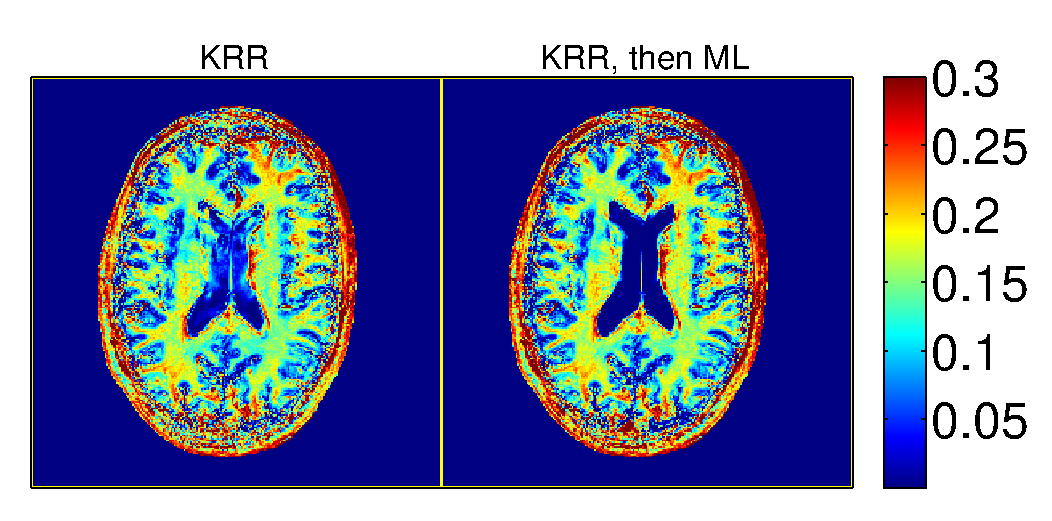
\includegraphics [height=7.4cm, clip] {ff,log2c-0,krr-ml}
    \end{minipage}
    
    \begin{minipage}[b]{0.96\textwidth}
        \centering
        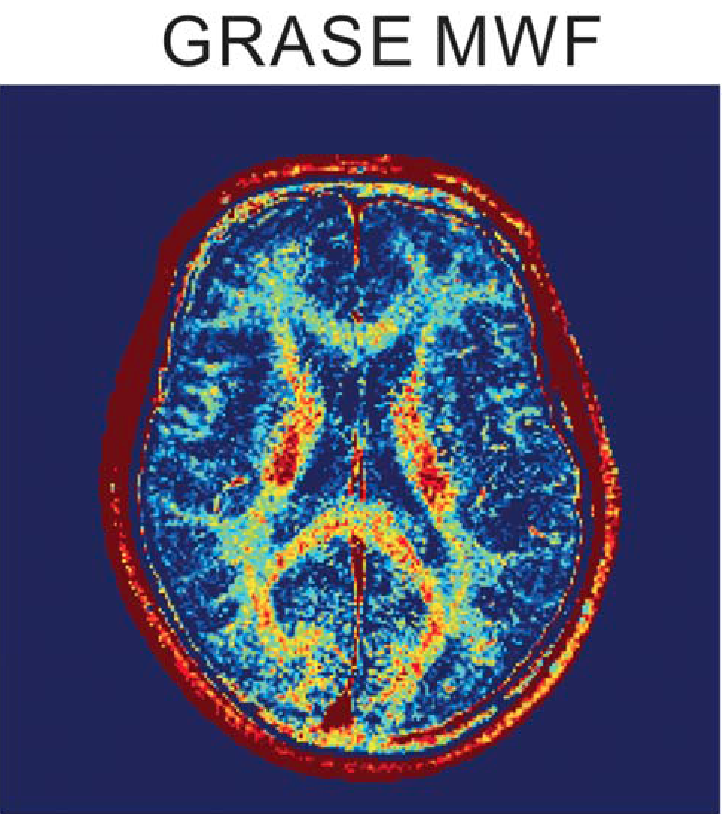
\includegraphics [height=7cm] {mwf,grase}
        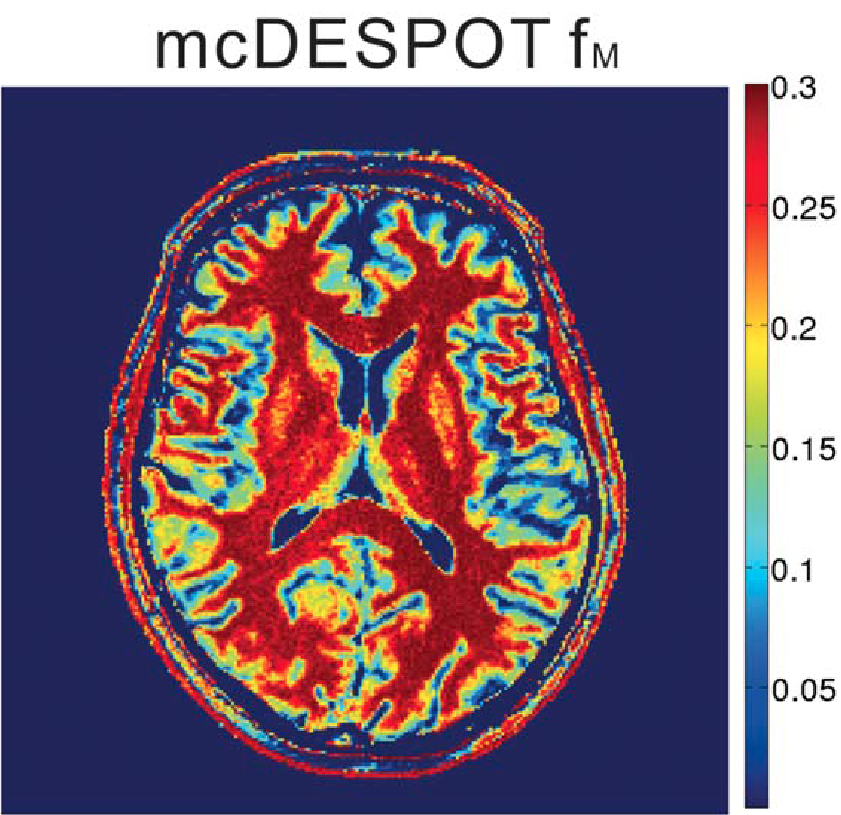
\includegraphics [height=7cm] {mwf,mcdespot}
    \end{minipage}
    \caption{
    	MWF estimates, using:
			our optimized SPGR/DESS scan profile
			and (\emph{top left}) KRR $\ff$ estimation,
			followed by (\emph{top right}) iterative ML estimation;
    	(\emph{bottom left})
			GRASE \cite{prasloski:12:rwc},
			a state-of-the-art acceleration
			to the slow gold-standard MESE acquisition
			originally used in \cite{mackay:94:ivv};
			and (\emph{bottom right})
			mcDESPOT \cite{deoni:11:com},
			a fast steady-state acquisition
			that lacks sufficient estimation precision \cite{lankford:13:oti}.
			All MWF estimates are from healthy volunteers,
			but those from GRASE/mcDESPOT
			are from a separate study
			in a different subject 
			and are reprinted 
			from \cite{zhang:15:com},
			a recent comparison study.
			The proposed precision-optimized SPGR/DESS scan profile
			is as fast as mcDESPOT
			and yields MWF images
			comparable to those of GRASE.
    }
    \label{fig:mwf,brain}
\end{figure}

Figure~\ref{fig:mwf,brain} compares resulting $\ff$ estimates 
using KRR only 
versus KRR followed by iterative ML estimation.
ML iterations produce visible improvement
in cerebrospinal fluid 
but leave $\ff$ estimates 
in WM and GM ROIs
largely unchanged.

For qualitative comparison,
Figure~\ref{fig:mwf,brain} also reprints
from a comparison study \cite{zhang:15:com}
MWF proxy estimates
from two other acquisitions:
GRASE \cite{prasloski:12:rwc}, 
a state-of-the-art acceleration
to the slow gold-standard MESE acquisition \cite{mackay:94:ivv};
and 
mcDESPOT \cite{deoni:11:com},
a faster steady-state acquisition
that lacks sufficient estimation precision \cite{lankford:13:oti}.
These images are from a separate study
of a different healthy volunteer,
and utilize different algorithms
to estimate different MWF proxies
from multi-compartmental signal models 
of different acquisitions.
Acknowledging the lack of controls,
we cautiously observe
that the proposed optimized SPGR/DESS scan profile
is as fast as the mcDESPOT acquisition
(controlling for scanner timing limitations)
and yields MWF maps
at least comparable in WM to those of GRASE.

\begin{table*} [tb]
	\centering
	\begin{minipage}{0.3\textwidth}
		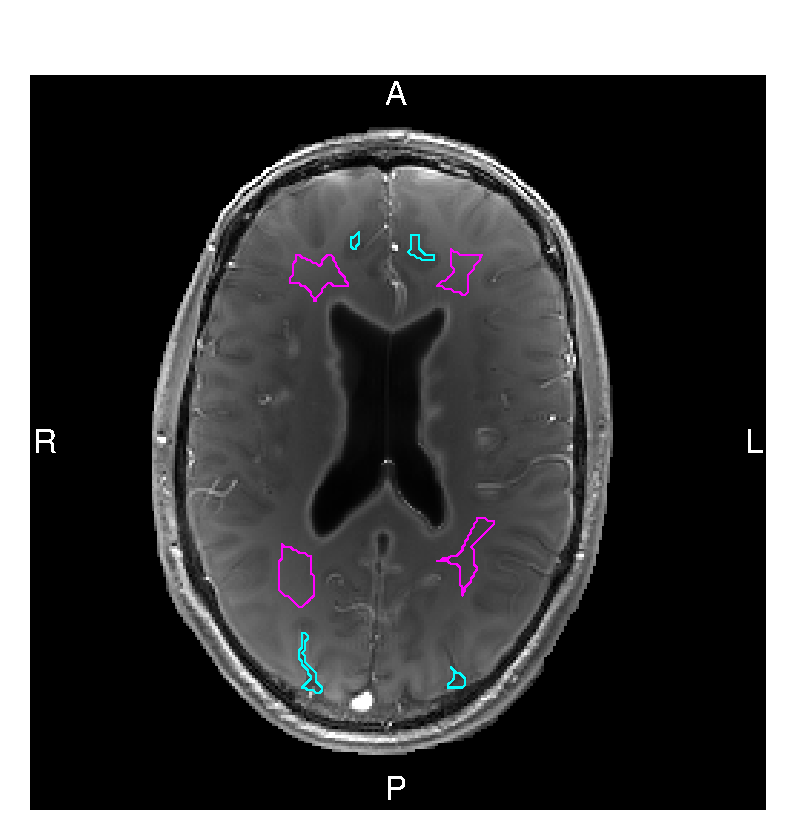
\includegraphics [width=4cm] {roi.eps}
		\label{fig:mwf,brain,roi}
	\end{minipage}
	\begin{minipage}{0.6\textwidth}
		\begin{tabu} {c | r r}
			\hline
			\hline
			ROI (\# voxels) & KRR & KRR, then ML \\
			\hline
			\WM \ffest ($725$) 	& \mnstd{0.130}{0.074} & \mnstd{0.134}{0.070} \\
			\GM \ffest ($176$)	& \mnstd{0.063}{0.106} & \mnstd{0.063}{0.098} \\
			\hline
			\hline
		\end{tabu}
	\end{minipage}
	\caption{
		\emph{Left}:
		\WM/\GM ROIs,
		overlaid on a representative anatomical
		(coil-combined SPGR) image.
		Four \WM ROIs and four \GM ROIs are each pooled
		into a single \WM and a single \GM ROI,
		over which sample statistics are computed.
		\emph{Right}:
		Within-ROI sample means $\pm$ 
		within-ROI sample standard deviations
		of $\ff$ estimates,
		using KRR only 
		as well as KRR with ML refinement
		(Fig.~\ref{fig:mwf,brain} presents corresponding images).
	}
	\label{tab:mwf,brain}
\end{table*}

% tab:mwf,brain summarizes within-roi sample means and sstd
% computed over 4 wm , 4 gm rois containing x voxels
% agree well with grase wm histograms (see fig. 5 in zhang:15:com for example)
% difficult to compare gm values given very high std dev
% however, grase did report mean about 0.05 in both cortical and internal gray matter
Table~\ref{tab:mwf,brain} summarizes 
within-ROI samples means and sample standard deviations
computed over manually-selected ROIs 
containing $725$ WM and $176$ GM voxels.
Compared to its KRR initialization,
local ML optimization
does not appreciably change 
WM/GM \ffest sample means
and mildly reduces sample standard deviations.
Our WM \ffest sample means
agree well with literature MESE measurements
(\eg, see \cite[Fig.~3]{zhang:15:com}).
Our GM \ffest sample means
are not statistically meaningful
because of high within-ROI sample variation,
likely due to the common challenge
of poor GM ROI selection.
Nevertheless,
it warrants mention 
that MWF in healthy GM 
was reported in \cite[Fig.~3]{zhang:15:com}
to be about $0.05$ using GRASE.

%%%%%%%%%%%%%%%%%%%%%%%%%%%%%%%%%%%%%%%%%%%%%%%%%%%
\section{Summary and Future Work}
\label{s,mwf,summ}
%%%%%%%%%%%%%%%%%%%%%%%%%%%%%%%%%%%%%%%%%%%%%%%%%%%

This chapter describes initial work 
on developing a fast steady-state acquisition
for precise MWF imaging.
We have thus far developed
a two-compartment signal model 
for the DESS pulse sequence;
used a simple non-exchanging version 
of this model 
(along with a similar SPGR model
from literature)
to design a fast scan profile
for precisely estimating 
fast-relaxing compartmental fraction $\ff$
as a proxy for MWF;
and applied this precision-optimized acquisition
\invivo to produce to our knowledge the first MWF images 
from combinations of fast SPGR/DESS scans.
Though preliminary results appear qualitatively comparable
in healthy WM
to state-of-the-art literature MESE results,
thorough validation is required
and will constitute a major portion 
of future work,
discussed in the following.

% need to first build support for claim that ff as measured by spgr/dess 
% is a measure of mwf as measured originally by mackay
% need to compare our estimates with estimates from a mese measurement
% foreseen challenges: still will be differences in model assumptions and estimation algorithms
\paragraph{Comparisons with MESE MWF Estimates}
We would like to claim
that fast-relaxing fraction $\ff$ estimates
from precision-optimized SPGR/DESS scan profiles
are accurate measurements 
of MWF as originally defined 
in \cite{mackay:94:ivv}.
To build support
for this hypothesis,
we will need
to systematically compare our $\ff$ estimates
with MWF estimates
from a MESE acquisition.
Such comparison is challenging
because the methods differ
not only in acquisitions
but also in modeling assumptions
\footnote{MESE MWF estimation 
	assumes $\To$ is known and fixed
	over many compartments.
	As presented, SPGR/DESS $\ff$ estimation
	assumes unknown variable $\To$
	across two compartments.
	Both models neglect exchange 
	and multi-compartmental off-resonance effects,
	and assume known flip angle spatial variation.
	\label{foot:mwf,assumption}
},
initialization
(KRR estimate \eqref{eq:krr,x-hat}
versus the zero vector),
objective functions
(ML cost \eqref{eq:relax,lf-mtx}
versus a regularized nonnegative least-squares (NNLS) cost
\cite[Eq.~8]{whittall:89:qio}),
and estimation algorithms
(gradient projection method \cite{rosen:60:tgp}
versus
least-distance programming (LDP) \cite[\S23.4]{lawson:74}).

% first validate krr by comparing mwf estimates from nnls/ldp vs krr, using same model
% then take as many assumptions same as possible while comparing mese and spgr/dess
% modify model (possibly of both acq) as needed to achieve agreement
We plan to approach validation as follows.
First,
we will compare \invivo MWF estimates
from a fixed signal model
of a fixed MESE acquisition
using KRR, KRR-initialized ML,
KRR-initialized regularized NNLS,
and zero-initialized regularized NNLS
\footnote{Both KRR- and zero-initialized NNLS 
	should yield near-equivalent solutions
	because the regularized NNLS problem is convex,
	assuming as in \cite{whittall:89:qio, mackay:94:ivv}
	that all latent parameters other than MWF are known.
}.
Here, 
all three iterative algorithms can be solved
via gradient projection method
for consistency.
These results will provide direct insight
as to how KRR and KRR-initialized ML estimation perform
for \invivo MWF estimation
from a classical acquisition and signal model.
% mese takes t1 as known as and constant across compartments from IR-prepared FSE sequences
% we estimate t1 for two compartments
% joint estimation of refocusing flip angle; we assume flip angle scaling known

% little bit of a trivial problem above (linear)
% next study nonlinear but relatively simple problem mwf and flip estimation
% t1 still known
% can't use nnls but can use krr and varpro 
% classical acquisition but more complicated signal model
Using KRR as above
for a convex MWF estimation problem 
is important for systematic validation
but is overkill in practice.
For a more interesting usage,
we will next consider joint estimation
of MWF and transmit field variation $\stx$
(still assuming knowledge of other latent parameters)
from the same MESE dataset.
NNLS is inapplicable 
for this non-convex problem;
however, 
we can still quickly validate KRR estimates 
via voxel-wise exhaustive grid search
due to low problem dimensionality.
If promising,
these results will support the claim
that KRR could be useful 
for fast \invivo MWF estimation 
from nonlinear models.

% next, could fix model assumptions 
% design spgr/dess acquisition for estimating ff from much simpler model
% this model will again lead to convex problem in ff that can be solved via above methods
% positive result here suggests that spgr/dess can be used to design mwf acquisitions
To compare SPGR/DESS and MESE acquisitions,
we can modify SPGR/DESS model assumptions
to those taken in \cite{prasloski:12:rwc}
for the MESE model
(listed in Footnote~\ref{foot:mwf,assumption})
and thereby formulate an analogous
$\Tt$ distribution estimation problem,
for which linear algorithms 
such as regularized NNLS and LDP are applicable.
Our task will then be 
to design a fast SPGR/DESS acquisition
under these modified model assumptions
that permits precise voxel-wise estimation 
of the $\Tt$ distribution.
The resulting estimated $\Tt$ distributions
will be directly comparable 
to $\Tt$ distributions 
from MESE acquisitions
and could be used
to form SPGR/DESS MWF maps
that are directly comparable 
with MESE MWF maps.

% finally, show true generality of methods developed in thesis
% can relax some model assumptions, design corresponding scans, and study via krr/ml only
% e.g., variable t1 over two discrete compartments gives acquisition in table mwf,acq
% others might be three discrete compartments or exchange (though this is hard w/ acq design)
% comparing with KRR-ML spgr/dess gives info about effect of model assumptions
Upon isolated validation
of acquisitions, initializations, and estimation algorithms,
we can explore the effects 
of different modeling assumptions
using the full flexibility
of optimized scan design and KRR estimation.
As a first experiment,
we could try to optimize
under the variable-$\To$ two-compartment model 
a MESE acquisition
similar to the SPGR/DESS acquisition 
presented in Table~\ref{tab:mwf,acq}
and compare resulting SPGR/DESS and MESE \ffest maps. 
If \ffest from these models do not measure MWF
with sufficient specificity,
we could explore similar comparisons
using more complicated models
involving exchange, three (or more) compartments,
and/or compartmental off-resonance effects.
All of these model comparisons 
will require highly nonlinear estimation problems
involving many latent parameters,
for which KRR-initialized ML estimation is well-suited.

% comparison with mt
% different measure of myelination - does it correlate?
\paragraph{Comparisons with Different Myelin Biomarkers}
We are also interested
in how $\ff$ estimates (or other MWF proxies)
correlate with other myelin biomarkers. 
One contending noninvasive marker arises
from MR pulse sequences sensitized
to the inhomogeneous magnetization transfer (ihMT) effect
\cite{varma:15:mtf},
which has recently been argued
to be specific
to the large membrane lipids
that comprise much of myelin
\cite{varma:15:iom, swanson:17:mda}.
Outside MRI,
invasive measurements
from histology
have been used to study myelin 
(as in \eg, \cite{gareau:00:mta, webb:03:imt})
and could serve as a gold-standard \insitu marker.
Multi-compartmental and ihHT MRI markers 
can be successively compared 
through phantom, healthy volunteer, and patient studies.
Both MRI and histological markers
can be compared through 
phantom and \insitu studies.
All of these studies
are highly amenable 
to clinical collaborations.
